%%%%%%%%%%%%Outline%%%%%%%%%%%%%%%%%%

% ==== opening: the three research questions ====
%%%
% message<the evaluation asks three questions: localization, attribution, and repair usefulness>
% we evaluate \sys with three questions
% RQ1 asks whether \sys localizes the proof break better than trusting the rejected line
% RQ2 asks whether \sys assigns the correct failure class and beats a message-level baseline
% RQ3 asks whether the structured diagnostic helps a developer repair the program

% ==== Setup ====
%%%
% message<bpfix-bench is a replay-disciplined corpus with independent tiered labels and three baselines>
% we evaluate on bpfix-bench, 235 rejections reproduced under one pinned environment
% the cases come from stack overflow 86, selftests 85, github commits 46, and issues 18
% labels are hand-assigned from separate evidence, the classifier playing no part, so they stay independent
% ground truth is tiered: 235 reproduce, 130 have an instruction-level root-cause index, 9 are adjudicated
% we compare against three baselines: last-line localizer, message dictionary, and raw-log repair

% ==== RQ1: Localizing the proof break ====
%%%
% message<the rejected line diverges from the cause per class, so the last-line baseline misses the hard classes; \sys's accuracy is pending>
% a useful localizer must point at where the proof broke, which can differ from the rejected instruction
% the table measures per class how often the root-cause index differs from the rejected index over 130 cases
% the two differ for 19% source bugs, 33% lowering, 3/3 false positives, 0/5 environment, gap at most 13
% the last-line baseline localizes source bugs well but misses the hard classes
% \sys's own localization accuracy against this baseline is pending a fresh replay capture

% ==== RQ2: Attributing the failure class ====
%%%
% message<\sys attributes the layer with heuristic signals; the measured comparison to a message baseline is pending>
% attribution assigns each rejection the layer that must change, scored over 235 cases against the message dictionary
% \sys reads 73 hand-written signals, and the false-positive verdict rests on only two precision signals, the weakest part
% the message dictionary cannot recover lowering artifacts or false positives, which share messages with source bugs
% the measured accuracy and confusion matrix are pending a fresh replay capture

% ==== RQ3: Helping repair ====
%%%
% message<bpfix-test shows that the structured diagnostic improves executable LLM repair>
% to test downstream use we build bpfix-test, 75 source-level repair cases with executable oracles
% the cases combine mechanism-designed programs and minimized real/tutorial seeds, and cover five verifier-failure mechanisms
% an oracle passes only when the candidate compiles, loads, and satisfies functional and source-semantics checks
% on Qwen3.6 27B, raw-log repair passes 22 of 75 and structured-diagnostic repair passes 38 of 75; with one retry they reach 30 and 44

% ==== Threats to validity ====
%%%
% message<pending captures, small samples, single-adjudicator labels, working-suite status, and corpus skew bound the results>
% the two pending results need every case's replay log, of which only one is in the artifact
% the hard classes carry few cases, reported with raw counts
% the adjudicated labels rest on a single adjudicator with agreement not yet measured
% the repair suite is a working suite rather than a frozen heldout benchmark
% the distance metric covers only the 130 same-numbering cases, and the source-bug skew bounds the rarer classes

%%%%%%%%%%%%Outline%%%%%%%%%%%%%%%%%%

\section{Evaluation}
\label{sec:evaluation}

We evaluate \sys with three research questions:
\begin{itemize}
  \item \textbf{RQ1 (localization).} Does \sys localize the instruction where the proof breaks more accurately than a baseline that trusts the rejected line?
  \item \textbf{RQ2 (attribution).} Does \sys assign the correct failure class, and does it beat a message-level baseline on the hard classes?
  \item \textbf{RQ3 (usefulness).} Does \sys's structured diagnostic help a developer repair the program?
\end{itemize}

\noindent\textbf{Setup.} We evaluate on \emph{bpfix-bench}, a corpus of 235 verifier rejections that each build, load, are rejected, and capture a level-two trace under one pinned environment (kernel 6.15.11 and clang 18.1.3). The cases come from Stack Overflow (86), kernel selftests (85), GitHub commits (46), and GitHub issues (18). Each case's root-cause instruction and taxonomy class are hand-assigned from separate evidence, with the \sys classifier playing no part, so the labels stay independent of the tool they evaluate. Ground truth is tiered: all 235 reproduce as artifacts, 130 carry an instruction-level root-cause index on the replay numbering, and 9 carry adjudicated class labels. We compare \sys against three baselines: a last-line localizer that returns the rejected instruction, a message dictionary that maps the terminal message to a class, and one-shot repair from the raw verifier log.

\noindent\textbf{RQ1: Localizing the proof break.} A useful localizer must point at where the proof broke, which can differ from the rejected instruction. Table~\ref{tab:rejection-cause-gap} measures, per class, how often the labeled root-cause instruction differs from the rejected instruction over the 130 instruction-localizable cases. The two differ for 19\% of source bugs and 33\% of lowering artifacts, for all 3 verifier false positives, and for none of the 5 environment cases, and the gap reaches at most 13 instructions. The last-line baseline therefore localizes source bugs well but misses the hard classes, where the rejected line and the cause carry different classes. \sys's own localization accuracy against this baseline, scored as exact and within-$k$ root-cause hits, is pending a fresh replay capture.

\input{tables/sec-5-cause-gap}

\noindent\textbf{RQ2: Attributing the failure class.} Attribution assigns each rejection the layer that must change, scored against the hand-assigned label over all 235 cases and compared to the message dictionary. \sys reads 73 hand-written signals over the rich trace to make this call, and the false-positive verdict rests on only two precision signals, so attribution is the weakest part of the system. The message dictionary cannot recover the lowering-artifact and false-positive classes, since they share terminal messages with source bugs. The measured comparison, an accuracy and per-class confusion matrix, is pending a fresh replay capture, because the per-case replay logs the scorer needs are not yet in the artifact.

\noindent\textbf{RQ3: Helping repair.} To test whether the structured diagnostic helps downstream repair, we build \emph{bpfix-test}, a 75-case source-level LLM repair suite with executable oracles. Each case contains a buggy BPF C program, the raw verifier log, the \sys diagnostic for the same rejection, a reference repair used only for admission checks, and a per-case oracle. The suite is organized by source family rather than by historical split: mechanism-designed standalone programs (40), Cilium (7), ActPlane (5), xdp-tools (5), AgentSight (4), bpf-developer-tutorial (4), bpftime (3), eunomia.dev (3), DatRail (2), NCCL-eBPF (1), and Tetragon (1). The cases cover proof-lifecycle loss, modern BPF protocol misuse, source/object correlation failures, helper memory contracts, and environment or configuration boundaries. A candidate passes only if it compiles, loads through the verifier, and satisfies the case's functional, proof-shape, source-semantics, and custom predicates; the model sees only the buggy source and either the raw log or the \sys diagnostic.

\begin{figure}[H]
  \centering
  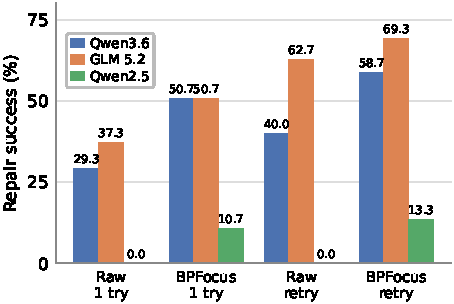
\includegraphics[width=\columnwidth]{figures/sec-5-bpfix-test.pdf}
  \caption{\testset repair success across three models. Bars are grouped by prompt mode, and color identifies the model. Retry bars use one failure-informed retry. \sys improves one-shot repair for all three models and remains ahead under retry.}
  \Description{A grouped bar chart compares raw verifier-log prompts and BPFix diagnostic prompts for Qwen3.6 27B, GLM 5.2, and Qwen2.5 3B. Each model has a distinct color. BPFix improves one-shot and retry pass rates for all three models.}
  \label{fig:bpfix-test}
\end{figure}


Figure~\ref{fig:bpfix-test} summarizes the paired prompt results across the three tested models. Under the same Qwen3.6 27B model, temperature, prompt budget, timeout, and oracle, one-shot repair from the raw verifier log passes 22 of 75 cases, while repair from the \sys diagnostic passes 38 of 75. Allowing one failure-informed retry raises the raw-log result to 30 of 75 and the \sys result to 44 of 75. This shows that \sys improves the first repair signal and that the advantage remains after an ordinary retry loop. A hosted GLM 5.2 check shows the same one-shot direction, 28 to 38 of 75, but retry narrows the gap, 47 to 52 of 75, indicating that retry is a strong intervention for that model. A small local Qwen2.5 3B stress run passes 0 of 75 from raw logs and 8 of 75 with \sys, so the suite also separates model capacity from diagnostic help. These results support a controlled-usefulness claim for the current working suite; they do not by themselves make \emph{bpfix-test} a frozen heldout benchmark.

\noindent\textbf{Threats to validity.} The two pending results, \sys's localization accuracy and the attribution confusion matrix, both need the per-instruction replay log of every case, and only one such log is in the artifact, so we will produce them from a fresh kernel-6.15.11 replay capture. The hard classes carry few cases, so we report them with raw counts. The 9 adjudicated labels rest on a single adjudicator, and inter-annotator agreement is not yet measured. The repair suite is a working suite built during benchmark development, not a frozen heldout benchmark; before making benchmark-generalization claims, we need a no-touch heldout split with complete source-family and mechanism metadata and clean reruns for every headline configuration. The instruction-distance metric is defined only on the 130 cases that share the replay numbering, and the corpus's skew toward source bugs, 194 of 235, bounds what the rarer classes can show.
